\section{Durchführung}
\label{sec:Durchführung}
Die in Abbildung \ref{fig:sus} zu sehende Schaltung wird zur Messung der Suszeptibilität genutzt.
Durch die Brückenschaltung kommt es zu Störspannungen, welche die Brückenspannung mitunter völlig überdecken. Es muss ein Selektiv-Verstärker zwischen der Brückenschaltung und dem Millivoltmeter eingebaut werden.
Dieser besteht aus einem filternden Teil und einem verstärkenden Teil. Dabei soll der Filter möglichst nur die für diesen Versuch benötigte monofrequente Signalspannung durchlassen und der Verstärker 
soll die geringe Brückenspannung verstärken.
\\
Im Folgenden soll zunächst der Filter untersucht werden, um die Güte des Selektiv-Verstärkers zu ermitteln.
Dazu wird ein Sinusspannungsgenerator an den Selektiv-Verstärker angeschlossen. An einem Millivoltmeter werden Messpaare der Ausgangsspannung in Abhängigkeit von der
Frequenz abgelesen. Die Frequenz wird in dem Bereich $\SI{20}{\kilo \hertz}$ bis $\SI{40}{\kilo \hertz}$ variiert. Dabei werden die Frequenzen in der Nähe des Maximum in kleineren Schritten gemessen.
Um die Suszeptibilität zu messen wird die in Abbildung \ref{fig:AU} zu sehende Apperatur aufgebaut.
\begin{figure}
    \centering
    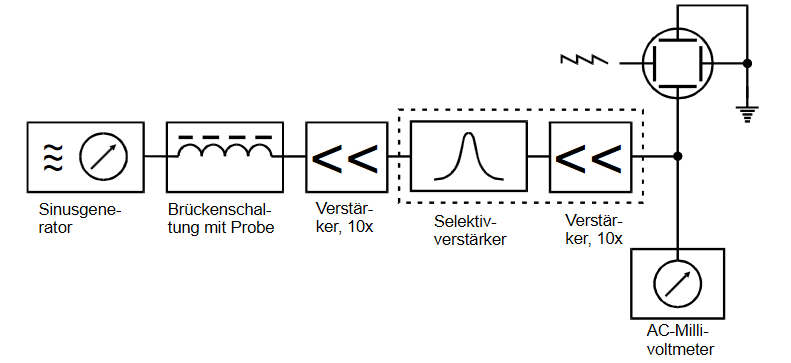
\includegraphics[scale=0.4]{pics/AU.png}
    \caption{Schaltbild zur Messung der Suszeptibilität. \cite{v606}}
    \label{fig:AU}
  \end{figure}
  Die Signalfrequenz des Sinusgenerators wird auf die Durchlassfrequenz des Selektiv-Verstärkers geregelt. Die Speisespannung wird am Sinusgenerator abgelesen und notiert.
  Bevor die Probe eingeführt wird, wird mit Hilfe des Abgleichelements die Brückenschaltung abgeglichen. Es werden die Werte der Brückenspannung $U_\text{Br}$ und des Abgleichelements $\sfrac{R_3}{R_4}$ notiert.
  Danach wird die Probe in die Spule eingesetzt. Die nach dem Abgleichen erreichte Brückenspannung und der zugehörige Wert des Abgleichelements werden notiert.
  Die Probe wird wieder aus der Spule genommen. Die Prozedur wird für jede Probe drei mal wiederholt. Als zu untersuchende Materialien stehen $\ce{Dy2 O3}$ und $\ce{Gd2 O3}$ zur Verfügung.
  Anschließend wird die Länge der Probe gemessen.